\begin{sectionbox}{El espectro electromagnético}
    Podemos clasificar y ordenar las ondas electromagnéticas de acuerdo a sus diferentes longitudes de onda y frecuencias; llamamos a esta clasificación \comillas{el espectro electromagnético}. La figura \ref{fig:01f944ab4471010d09766560f4d1c6da4846d97d} muestra este espectro, que consiste de todos las clases de radiación electromagnética que existen en nuestro universo.

    \begin{figure}[H]
        \centering
        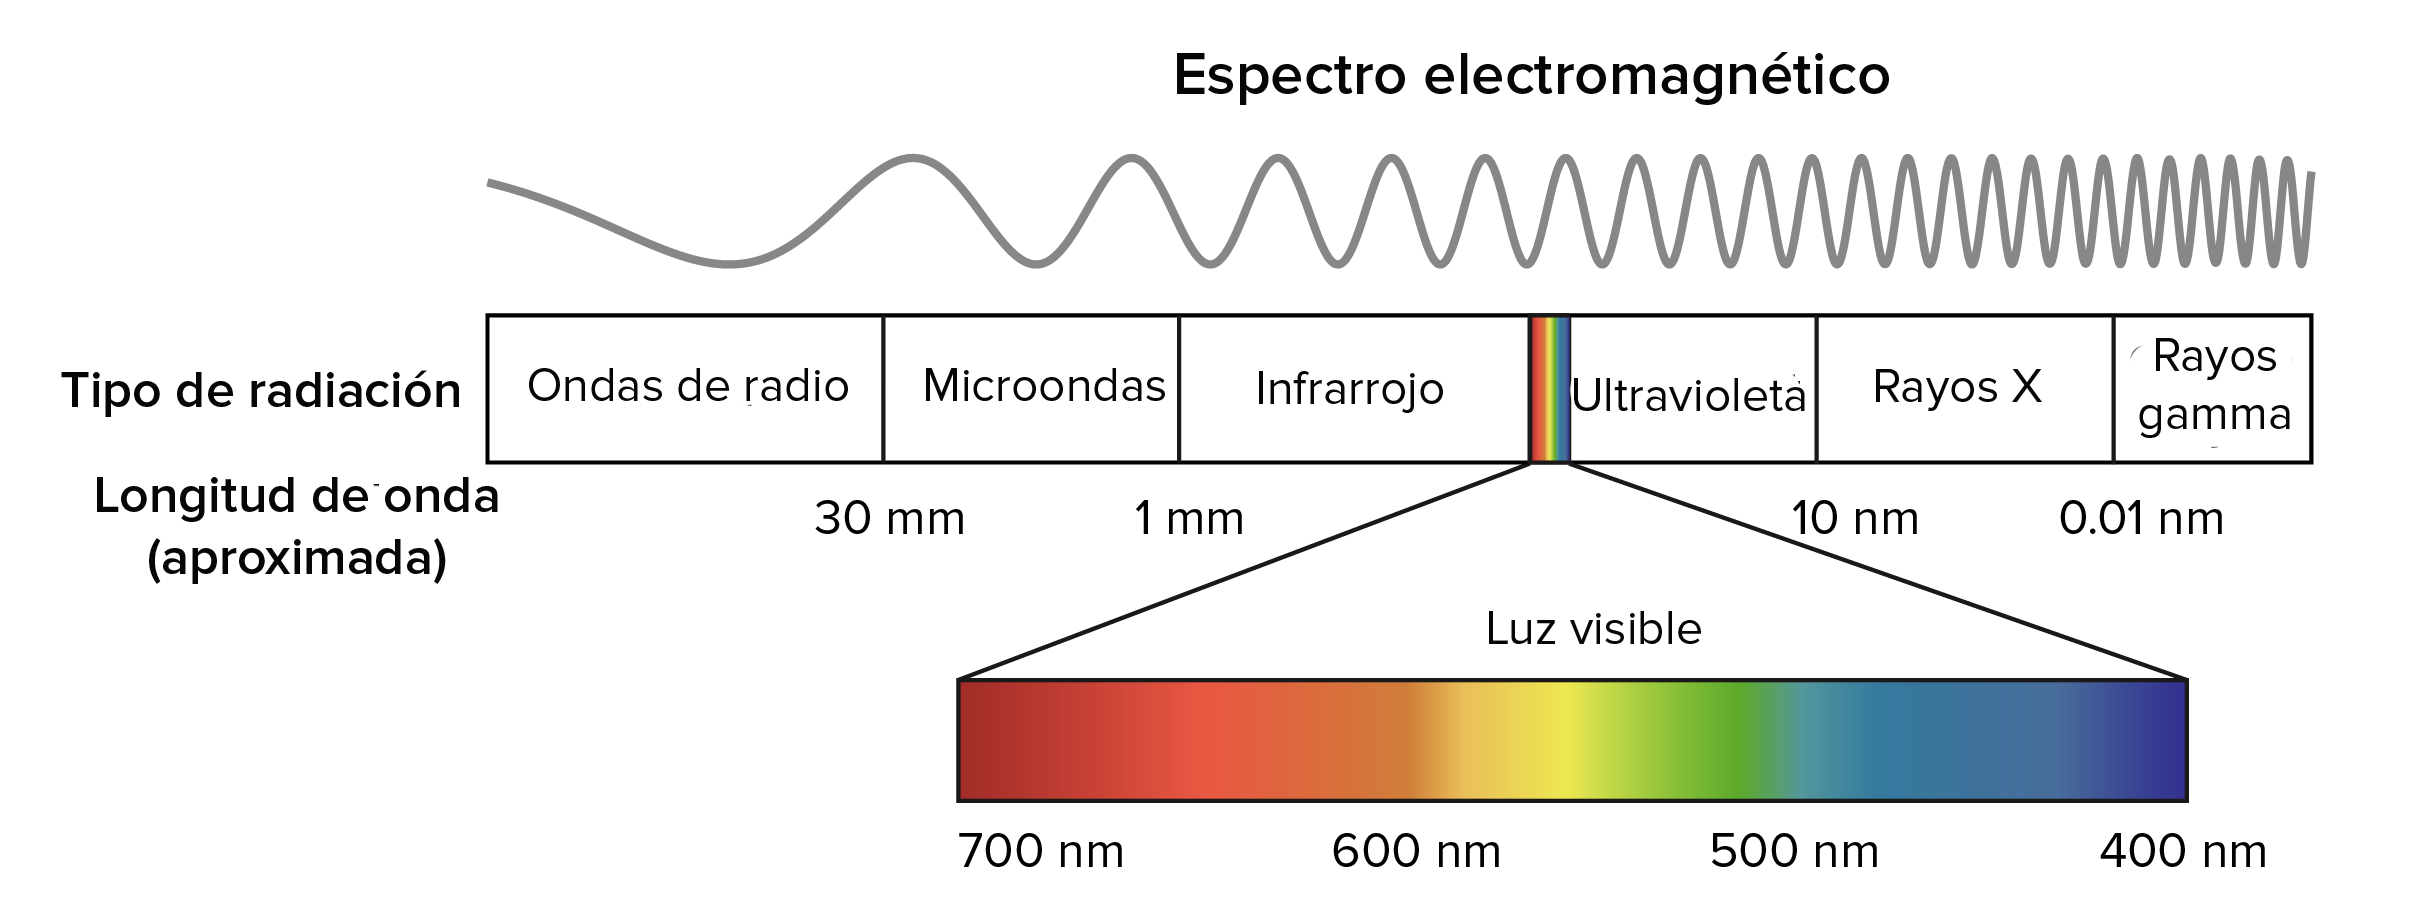
\includegraphics[width=0.9\linewidth]{../images/01f944ab4471010d09766560f4d1c6da4846d97d}
        \caption{El espectro electromagnético.}
        \label{fig:01f944ab4471010d09766560f4d1c6da4846d97d}
    \end{figure}

    Como podemos ver, el espectro visible —es decir, la luz que podemos ver con nuestros ojos— es tan solo una pequeña fracción de las diferentes clases de radiación que existen. A la derecha del espectro visible, encontramos las clases de energía que son menores en frecuencia (y por lo tanto mayores en longitud de onda) que la luz visible. Estas clases de energía incluyen los rayos infrarrojos (IR) (ondas de calor emitidas por los cuerpos térmicos), las microondas y las ondas de radio. Estos tipos de radiación nos rodean constantemente; no son dañinos, pues sus frecuencias son muy bajas. Como veremos en la sección siguiente, \comillas{El fotón}, las ondas de baja frecuencia tienen poca energía, y por lo tanto no son peligrosas para nuestra salud.
    A la izquierda de espectro visible, encontramos los rayos ultravioleta (UV), los rayos X y los rayos gamma. Estas clases de radiación son dañinas para los organismos vivos, pues tienen frecuencias extremadamente altas (y por lo tanto, mucha energía). Es por esta razón que usamos loción bloqueadora en la playa (para bloquear los rayos UV provenientes del sol) y que, para prevenir que los rayos X penetren otras áreas del cuerpo distintas de la que requiere visualizarse, un técnico de rayos X coloca una placa de plomo sobre nosotros. Los rayos gamma son los más dañinos, pues son los más altos en frecuencia y en energía. Afortunadamente, nuestra atmósfera absorbe los rayos gamma que provienen del espacio, y así nos protege del daño.
\end{sectionbox}